\documentclass[10pt,a4paper,oneside,fleqn]{article}
\usepackage{geometry}
\geometry{a4paper,left=20mm,right=20mm,top=1cm,bottom=2cm}
\usepackage[utf8]{inputenc}
%\usepackage{ngerman}
\usepackage{amsmath}                % brauche ich um dir Formel zu umrahmen.
\usepackage{amsfonts}                % brauche ich für die Mengensymbole
\usepackage{graphicx}
\setlength{\parindent}{0px}
\setlength{\mathindent}{10mm}
\usepackage{bbold}                    %brauche ich für die doppel Zahlen Darstellung (Einheitsmatrix z.B)
\usepackage{dsfont}          %F�r den Einheitsoperator \mathds 1


\usepackage{color}
\usepackage{titlesec} %sudo apt-get install texlive-latex-extra

\definecolor{darkblue}{rgb}{0.1,0.1,0.55}
\definecolor{verydarkblue}{rgb}{0.1,0.1,0.35}
\definecolor{darkred}{rgb}{0.55,0.2,0.2}

%hyperref Link color
\usepackage[colorlinks=true,
        linkcolor=darkblue,
        citecolor=darkblue,
        filecolor=darkblue,
        pagecolor=darkblue,
        urlcolor=darkblue,
        bookmarks=true,
        bookmarksopen=true,
        bookmarksopenlevel=3,
        plainpages=false,
        pdfpagelabels=true]{hyperref}

\titleformat{\chapter}[display]{\color{darkred}\normalfont\huge\bfseries}{\chaptertitlename\
\thechapter}{20pt}{\Huge}

\titleformat{\section}{\color{darkblue}\normalfont\Large\bfseries}{\thesection}{1em}{}
\titleformat{\subsection}{\color{verydarkblue}\normalfont\large\bfseries}{\thesubsection}{1em}{}

% Notiz Box
\usepackage{fancybox}
\newcommand{\notiz}[1]{\vspace{5mm}\ovalbox{\begin{minipage}{1\textwidth}#1\end{minipage}}\vspace{5mm}}

\usepackage{cancel}
\setcounter{secnumdepth}{3}
\setcounter{tocdepth}{3}





%-------------------------------------------------------------------------------
%Diff-Makro:
%Das Diff-Makro stellt einen Differentialoperator da.
%
%Benutzung:
% \diff  ->  d
% \diff f  ->  df
% \diff^2 f  ->  d^2 f
% \diff_x  ->  d/dx
% \diff^2_x  ->  d^2/dx^2
% \diff f_x  ->  df/dx
% \diff^2 f_x  ->  d^2f/dx^2
% \diff^2{f(x^5)}_x  ->  d^2(f(x^5))/dx^2
%
%Ersetzt man \diff durch \pdiff, so wird der partieller
%Differentialoperator dargestellt.
%
\makeatletter
\def\diff@n^#1{\@ifnextchar{_}{\diff@n@d^#1}{\diff@n@fun^#1}}
\def\diff@n@d^#1_#2{\frac{\textrm{d}^#1}{\textrm{d}#2^#1}}
\def\diff@n@fun^#1#2{\@ifnextchar{_}{\diff@n@fun@d^#1#2}{\textrm{d}^#1#2}}
\def\diff@n@fun@d^#1#2_#3{\frac{\textrm{d}^#1 #2}{\textrm{d}#3^#1}}
\def\diff@one@d_#1{\frac{\textrm{d}}{\textrm{d}#1}}
\def\diff@one@fun#1{\@ifnextchar{_}{\diff@one@fun@d #1}{\textrm{d}#1}}
\def\diff@one@fun@d#1_#2{\frac{\textrm{d}#1}{\textrm{d}#2}}
\newcommand*{\diff}{\@ifnextchar{^}{\diff@n}
  {\@ifnextchar{_}{\diff@one@d}{\diff@one@fun}}}
%
%Partieller Diff-Operator.
\def\pdiff@n^#1{\@ifnextchar{_}{\pdiff@n@d^#1}{\pdiff@n@fun^#1}}
\def\pdiff@n@d^#1_#2{\frac{\partial^#1}{\partial#2^#1}}
\def\pdiff@n@fun^#1#2{\@ifnextchar{_}{\pdiff@n@fun@d^#1#2}{\partial^#1#2}}
\def\pdiff@n@fun@d^#1#2_#3{\frac{\partial^#1 #2}{\partial#3^#1}}
\def\pdiff@one@d_#1{\frac{\partial}{\partial #1}}
\def\pdiff@one@fun#1{\@ifnextchar{_}{\pdiff@one@fun@d #1}{\partial#1}}
\def\pdiff@one@fun@d#1_#2{\frac{\partial#1}{\partial#2}}
\newcommand*{\pdiff}{\@ifnextchar{^}{\pdiff@n}
  {\@ifnextchar{_}{\pdiff@one@d}{\pdiff@one@fun}}}
\makeatother
%
%Das gleich nur mit etwas andere Syntax. Die Potenz der Differentiation wird erst
%zum Schluss angegeben. Somit lautet die Syntax:
%
% \diff_x^2  ->  d^2/dx^2
% \diff f_x^2  ->  d^2f/dx^2
% \diff{f(x^5)}_x^2  ->  d^2(f(x^5))/dx^2
% Ansonsten wie Oben.
%
%Ersetzt man \diff durch \pdiff, so wird der partieller
%Differentialoperator dargestellt.
%
%\makeatletter
%\def\diff@#1{\@ifnextchar{_}{\diff@fun#1}{\textrm{d} #1}}
%\def\diff@one_#1{\@ifnextchar{^}{\diff@n{#1}}%
%  {\frac{\textrm d}{\textrm{d} #1}}}
%\def\diff@fun#1_#2{\@ifnextchar{^}{\diff@fun@n#1_#2}%
%  {\frac{\textrm d #1}{\textrm{d} #2}}}
%\def\diff@n#1^#2{\frac{\textrm d^#2}{\textrm{d}#1^#2}}
%\def\diff@fun@n#1_#2^#3{\frac{\textrm d^#3 #1}%
%  {\textrm{d}#2^#3}}
%\def\diff{\@ifnextchar{_}{\diff@one}{\diff@}}
%\newcommand*{\diff}{\@ifnextchar{_}{\diff@one}{\diff@}}
%
%Partieller Diff-Operator.
%\def\pdiff@#1{\@ifnextchar{_}{\pdiff@fun#1}{\partial #1}}
%\def\pdiff@one_#1{\@ifnextchar{^}{\pdiff@n{#1}}%
%  {\frac{\partial}{\partial #1}}}
%\def\pdiff@fun#1_#2{\@ifnextchar{^}{\pdiff@fun@n#1_#2}%
%  {\frac{\partial #1}{\partial #2}}}
%\def\pdiff@n#1^#2{\frac{\partial^#2}{\partial #1^#2}}
%\def\pdiff@fun@n#1_#2^#3{\frac{\partial^#3 #1}%
%  {\partial #2^#3}}
%\newcommand*{\pdiff}{\@ifnextchar{_}{\pdiff@one}{\pdiff@}}
%\makeatother

%-------------------------------------------------------------------------------
%%Nützliche Makros um in der Quantenmechanik Bras, Kets und das Skalarprodukt
%%zwischen den beiden darzustellen.
%%Benutzung:
%% \bra{x}  ->    < x |
%% \ket{x}  ->    | x >
%% \braket{x}{y} ->   < x | y >



\newcommand\bra[1]{\left\langle #1 \right|}
\newcommand\ket[1]{\left| #1 \right\rangle}
\newcommand\braket[2]{%
 \left\langle \vphantom{#2} #1%
   \middle|%
   \vphantom{#1} #2\right\rangle}%

%-------------------------------------------------------------------------------
%%Aus dem Buch:
%%Titel:  Latex in Naturwissenschaften und Mathematik
%%Autor:  Herbert Voß
%%Verlag: Franzis Verlag, 2006
%%ISBN:   3772374190, 9783772374197
%%
%%Hier werden drei Makros definiert:\mathllap, \mathclap und \mathrlap, welche
%%analog zu den aus Latex bekannten \rlap und \llap arbeiten, d.h. selbst
%%keinerlei horizontalen Platz benötigen, aber dennoch zentriert zum aktuellen
%%Punkt erscheinen.

\newcommand*\mathllap{\mathstrut\mathpalette\mathllapinternal}
\newcommand*\mathllapinternal[2]{\llap{$\mathsurround=0pt#1{#2}$}}
\newcommand*\clap[1]{\hbox to 0pt{\hss#1\hss}}
\newcommand*\mathclap{\mathpalette\mathclapinternal}
\newcommand*\mathclapinternal[2]{\clap{$\mathsurround=0pt#1{#2}$}}
\newcommand*\mathrlap{\mathpalette\mathrlapinternal}
\newcommand*\mathrlapinternal[2]{\rlap{$\mathsurround=0pt#1{#2}$}}

%%Das Gleiche nur mit \def statt \newcommand.
%\def\mathllap{\mathpalette\mathllapinternal}
%\def\mathllapinternal#1#2{%
%  \llap{$\mathsurround=0pt#1{#2}$}% $
%}
%\def\clap#1{\hbox to 0pt{\hss#1\hss}}
%\def\mathclap{\mathpalette\mathclapinternal}
%\def\mathclapinternal#1#2{%
%  \clap{$\mathsurround=0pt#1{#2}$}%
%}
%\def\mathrlap{\mathpalette\mathrlapinternal}
%\def\mathrlapinternal#1#2{%
%  \rlap{$\mathsurround=0pt#1{#2}$}% $
%}

%-------------------------------------------------------------------------------
%%Hier werden zwei neue Makros definiert \overbr und \underbr welche analog zu
%%\overbrace und \underbrace funktionieren jedoch die Gleichung nicht
%%'zerreißen'. Dies wird ermöglicht durch das \mathclap Makro.

\def\overbr#1^#2{\overbrace{#1}^{\mathclap{#2}}}
\def\underbr#1_#2{\underbrace{#1}_{\mathclap{#2}}}


\begin{document}
\tableofcontents
\setcounter{chapter}{3}
\chapter{Identische Teilchen}

\section{Fermionen \& Bosonen}

1 Teilchenzustand \(|K'\rangle \) K als kollektiver Index

2 Teilchenzustand \(|K'\rangle|K''\rangle \) oder \(|K''\rangle|K'\rangle \)

 \(|K'\rangle\neq |K''\rangle \) Orthogonal \(\Rightarrow \) \(|K'\rangle|K''\rangle \bot |K''\rangle|K'\rangle \) beschreiben gleiche Situation \(\rightarrow\) Austausch-Entartung

Lösung: Permutationssymmetrie unter Austausch identischer Teilchen. Permutationsoperator \(P_{ij}\)
 
\(|K'\rangle|K''\rangle...|K^{(n)}\rangle \) oder \(|1\rangle|2\rangle...|n\rangle \)

\begin{align}
P_{ij}&|K'\rangle ...|K\rangle|K^{(i+1)}\rangle ...|K^{(j)}\rangle ...
&=|K'\rangle ...|K^{i-1}\rangle|K^{(i)}\rangle|K^{(i+1)}\rangle ...|K^{(j)}\rangle ...
\end{align}

\[S_n = \{ P_\pi = \pi_{\{ij\}}P_{ij} \}\]

\(n!\) Permutationen von \(n\) Elementen \(\rightarrow dim S_n = n! \)

Eigenschaften: \(P^2_{ij}=1\), \(S_n\) nichtkommutativ für \(n\geq 3\)
\[P_{12}P_{23}|K'\rangle|K''\rangle|K'''\rangle= P_{12}|K'\rangle|K'''\rangle|K''\rangle= |K'''\rangle|K'\rangle|K''\rangle\]
\[P_{23}P_{12}|K'\rangle|K''\rangle|K'''\rangle= P_{23}|K''\rangle|K'\rangle|K'''\rangle= |K''\rangle|K'''\rangle|K'\rangle\]


\(P_{ij}\) und Observablen

\[A_1|a'\rangle |a''\rangle = a'|a'\rangle |a''\rangle\]
\[A_2|a'\rangle |a''\rangle = a''|a'\rangle |a''\rangle\]


Was ist \(P_{12}A_1P_{12}^{-1}\)

\[P_{12}A_1P_{12}^{-1}|a'\rangle |a''\rangle = P_{12}A_1 |a''\rangle |a'\rangle =  P_{12}a''|a''\rangle |a'\rangle = a'' P_{12}|a''\rangle |a'\rangle  = a''|a'\rangle |a''\rangle\]

\(P_{12}A_1 P_{12}^{-1} = A_2\), \(P_{ij}A_jP_{ij}^{-1}=A_i\)

Hamiltonoperator invariant unter Permutation identischer Teilchen

\[H= \frac{\vec p_1^2}{2m}+ \frac{\vec p_2^2}{2m} +V(\vec x_1)+ V(\vec x_2) + V_{pair}(|\vec x_1-\vec x_2|) \]

\[\Rightarrow P_{12}HP_{12}^{-1} = H \Leftrightarrow [H,P_{12}]=0\]


\(\Rightarrow \) Es gibt simultane Eigenzustände zu \(P_{12},H\)

\(P_{12}\) hat Eigenwerte \(\pm 1\)

\[+1: |K'K''\rangle_+=\frac{1}{\sqrt{2}}(|K'\rangle|K''\rangle + |K''\rangle|K'\rangle) \]
\[-1: |K'K''\rangle_-=\frac{1}{\sqrt{2}}(|K'\rangle|K''\rangle - |K''\rangle|K'\rangle) \]

Verallgemeinerung auf \(n\) Teilchen: irreduzible Darstellung  der \(S_n\). \(S_n\) hat 2 1-dimensionale Darstellungen. 

\begin{enumerate}
\item[a)] Symmetrische Darstellung \(\pi \to 1\)
\[|K'...K'''\rangle_+ = \frac{1}{\sqrt{n!}}\sum_{\pi\in S_n}1\cdot P_\pi |K'\rangle|K''\rangle...|K^{(n)}\rangle \]
Bosonen
\item[b)] Antisymmetische Darstellung \(\pi \to \delta=\begin{cases}
  +1 & \pi \text{ gerade,}\\
  -1 & \pi \text{ ungerade.}
\end{cases}\)
\[|K'...K'''\rangle_- = \frac{1}{\sqrt{n!}}\sum_{\pi\in S_n}\delta_\pi\cdot P_\pi |K'\rangle|K''\rangle...|K^{(n)}\rangle \]
Fermionen
\end{enumerate}




\underline{Bose-Einstein Statistik}

\[P_{ij}\underbrace{|\text{n identische Teilchen}\rangle}_{|K^{(1)}...K^{(n)}\rangle_+} = +|\text{n id.Teilchen}\rangle \]

\underline{Fermi-Dirac  Statistik}
\[P_{ij}\underbrace{|\text{n identische Teilchen}\rangle}_{|K^{(1)}...K^{(n)}\rangle_-} = -|\text{n id.Teilchen}\rangle \]

Bew.: 
\begin{align}
P_{ij}|K^{(1)}...K^{(n)}\rangle_-&=\frac{1}{\sqrt{n!}}\sum_{\pi\in S_n}\delta_\pi\underbrace{P_{ij}P_\pi}_{-P_{\pi_{ij}}} |K^{(1)}\rangle|K^{(2)}\rangle...|K^{(n)}\rangle \\
&=-\frac{1}{\sqrt{n!}}\sum_{\pi\in S_n}\delta_\pi P_{\pi_{ij}} |K^{(1)}\rangle|K^{(2)}\rangle ...|K^{(n)}\rangle \\
&=-|K^{(1)} ... K^{(n)}\rangle_{-}
\end{align}



Zusammenhang von Statistik und SpinTeilchen mit 
\begin{itemize}
\item Spin 0,1,2,... sind Bosonen
\item Spin \(\frac{1}{2},\frac{3}{2},\frac{5}{2}\)... sind Fermionen
\end{itemize}

Innerhalb relativistischer quantenfeldtheorie: 
\begin{itemize}
\item Spin-Statistik Theorem Spin \(\frac{1}{2}\)... Fermionen und Spin 0,1,... Bosonen. 
\item keine Para-Statistik, d.h. höhere irreduzible Darstellung der \(S_n\)
\end{itemize}

\subsection{2 Elektronen Systeme}

2 \(e^-\) können nicht den gleichen Zustand besetzen. 

\[(|K'\rangle |K'\rangle)_- = \frac{1}{\sqrt{2}}(1-P_{12})|K'\rangle |K'\rangle = 0\]

\underline{Pauli-Prinzip}
Basis Zustand: \(|\vec x_1\rangle |m_{s1}\rangle \otimes |\vec x_2\rangle |m_{s2}\rangle\)

Annahme: \([H,\vec S_{tot}]=0\)

\[\rightarrow |\psi\rangle = \phi (\vec x_1,\vec x_2)\chi (m_{s1},m_{s2})\]

\[|\psi\rangle  = \int d^3\vec x_1d^3\vec x_2\sum_{m_{s1}m_{s2}}\phi(\vec x_1,\vec x_2)\chi (m_{s1},m_{s2})|\vec x_1\rangle |m_{s1}\rangle |\vec x_2\rangle |m_{s2}\rangle \]

\(S^2_{tot}\) Eigenzustände

\[\chi(m_{s1},m_{s2})=\begin{cases}
  \chi_{++}(=\delta_{m_{s1}+\frac{1}{2}} \delta_{m_{s2}+\frac{1}{2}}) & S=1,\text{Triplett}\\
  \frac{1}{\sqrt{2}}(\chi_{+-}+\chi_{-+}) & S=1,\text{Triplett}\\
 \chi_{--} & S=1,\text{Triplett} \\
 \frac{1}{\sqrt{2}}(\chi_{+-}-\chi_{-+}) & S=0, \text{Singulett}\\
\end{cases}\]

Unter Permutation von 1 \(\leftrightarrow \) 2

\[P_{12}\chi_{\text{triplet}}= +\chi_{\text{triplet}} \Rightarrow \phi(\vec x_1,\vec x_2) = -\phi(\vec x_2,\vec x_1)\]
\[P_{12}\chi_{\text{Singulett}}= -\chi_{\text{Signulet}} \Rightarrow \phi(\vec x_1,\vec x_2) = +\phi(\vec x_2,\vec x_1)\]

Bsp:

\[H = \underbrace{\frac{\vec p_1^2}{2m}+V(\vec x_1)}_{H_1}+ \underbrace{\frac{\vec p_2^2}{2m}+V(\vec x_2)}_{H_2} \]

Mit \(H_{1}\omega_A(\vec x_1) = E_A\omega_A(\vec x_1)\)

\(H_{2}\omega_A(\vec x_2) = E_A\omega_A(\vec x_2)\)

folgen Lösungen für \(H|\psi\rangle =E|\psi\rangle \)

\[\psi\rangle = \omega_A(\vec x_1) \omega_B(\vec x_2) \chi\]

mit \(E= E_A+E_B\). Lösungen die Fermi-Dirac Statistik erfüllen

\[\phi(\vec x_1,\vec x_2) = \frac{1}{\sqrt{2}}(\omega_A(\vec x_1) \omega_B(\vec x_2) \pm \omega_B(\vec x_1) \omega_A(\vec x_2)) \]

\(+\) Für Singulett \(-\) für Triplett

Wahrscheinlichkeit

\begin{itemize}
\item Teilchen 1 bei \(\vec x_1\) in \(d^3\vec x_1\) und
\item Teilchen 2 bei \(\vec x_2\) in \(d^3\vec x_2\) zu finden
\end{itemize}


\begin{align}
&|\phi(\vec x_1,\vec x_2)|^2 d^3\vec x_1 d^3\vec x_2 =\\
&= \frac{1}{2}(|\omega_A(\vec x_1)|^2|\omega_B(\vec x_1)|^2+|\omega_B(\vec x_1)|^2|\omega_A(\vec x_1)|^2 \underbrace{ \pm 2Re\{\omega_A(\vec x_1) \omega_B(\vec x_2)\omega_A^*(\vec x_1) \omega_B^*(\vec x_2) \}}_{\text{Austausch-Dichte}}d^3\vec x_1d^3\vec x_2
\end{align}

\begin{enumerate}
\item[a)] Klassische Situation für A und B ohne Überlapp (Austauschdichte = 0)
\item[b)] Effekt der Statistik nur für starken Überlapp von A und B
\end{enumerate}


\subsection{He Atom}

Kern mit \(Z=2\), 2 \(e^-\)

\[H = \underbrace{\frac{\vec p_1^2}{2m}+ \frac{\vec p_2^2}{2m}-\frac{Ze^2}{4\pi \epsilon_0 r_1} -\frac{Ze^2}{4\pi \epsilon_0 r_2}}_{H_0}+\underbrace{\frac{e^2}{4\pi\epsilon_0 r_{12}}}_{V}\]

\(r_{12}=|\vec x_1-\vec x_2|\)

Eigenzustände von \(H_0\) sind Produkte von 'Wasserstoffzustände für \(Z=2\). z.B:

\[|K'\rangle |K''\rangle \equiv |100\rangle |nlm\rangle \]

\[\Rightarrow \phi(\vec x_1,\vec x_2) = \frac{1}{\sqrt{2}}(\psi_{100}(\vec x_1)\psi_{nlm}(\vec x_2)\pm \psi_{nlm}(\vec x_1)\psi_{100}(\vec x_2) ) \]

\[E^{(1)} = E_1+E_n \]

mit \(E_n = -Z^2\frac{e^2}{4\pi\epsilon_0 a_0}\frac{1}{2n^2}=-Z^2\cdot 13,6 eV\frac{1}{n^2}\)

Energie Shift

\[\Delta = \langle \frac{e^2}{4\pi\epsilon_0|\vec x_1-\vec x_2|} \rangle = I\pm J \]

\[I = \int d^3\vec x_1 d^3\vec x_2 |\psi_{100}(\vec x_1)|^2 |\psi_{nlm}(\vec x_2)|^2 \frac{e^2}{4\pi\epsilon_0|\vec x_1-\vec x_2|} \geq 0\]


\[J=\int d^3 \vec x_1 d^3 x_2\psi_{100}(\vec x_1)\psi_{nlm}(\vec x_2) \psi_{nlm}^*(\vec x_1)\psi_{100}(\vec x_2)\frac{e^2}{4\pi\epsilon_0|\vec x_1-\vec x_2|}\]

Für die Berechnung

\[\frac{1}{|\vec x_1-\vec x_2|}\approx \sum_{l,m}\frac{r^2_<}{r^{l+1}_>}Y_{lm}(\theta_1,\phi_1)Y_{lm}^*(\theta_2,\phi_2)\]

Spektrum von He


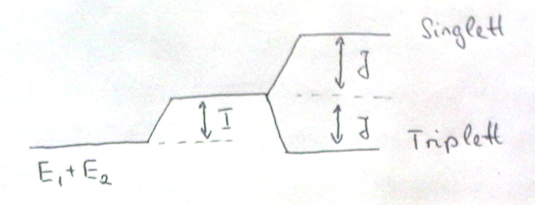
\includegraphics[width=0.75\textwidth]{kap04_01.png}

Ohne \(\vec S_1\cdot \vec S_2\) Kopplung tritt Spin Aufspaltung auf.

\(n=2,l=1\): \(I\approx 0.06eV\) und \(J\approx 0.13eV\)



\end{document}
